\documentclass{article}
\usepackage{graphicx}


\begin{document}

\title{CMSC 471: Project 2}
\author{Lee Brown}

\maketitle

\begin{figure}[h!]
  \centering
  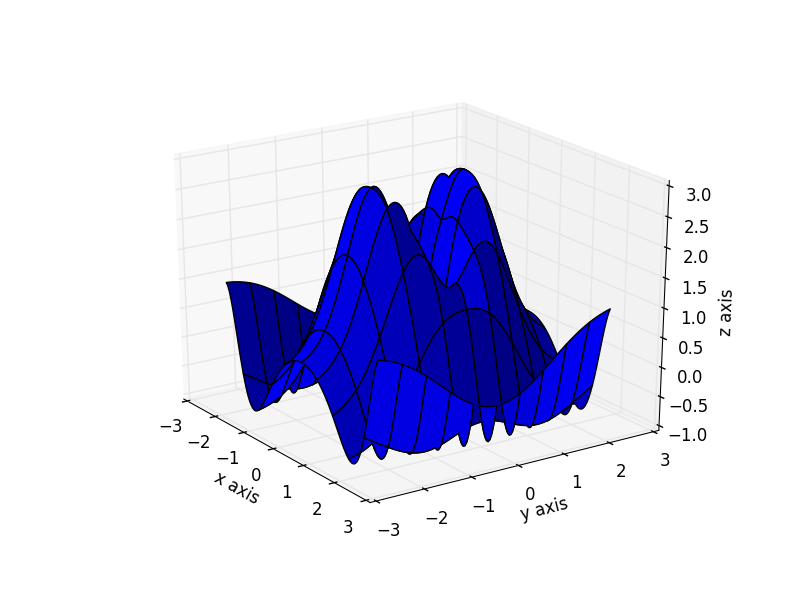
\includegraphics[scale=.5]{figure1.png}
  \caption{Image of Plotted Function}
\end{figure}

\section{Analysis of Methods}
Of the three methods used, hill climbing using random restarts was the most accurate. Without the random restarts, the hill climbing local search was unreliable to actually find good estimates for the global minimum. The random restarts made it more likely for the the search to yield more accurate results. However, this has drawbacks of its own. Hill climbing with random restarts requires a suitable sample size to yield accurate results. This causes the search to become increasingly inefficient and subsequently increasing the runtime. My test had it repeat hillclimbing 10,000 times, which caused a noticeable slowdown in run time, but also yielded more accurate results than the other tests.  

Simulated annealing was faster than hill climbing with random restarts, however without a very large cooldown time it doesn’t always yield accurate results. Due to the randomness involved, simulated annealing wasn’t always as accurate as hill climbing with random restarts.

\begin{figure}[h!]
  \centering
  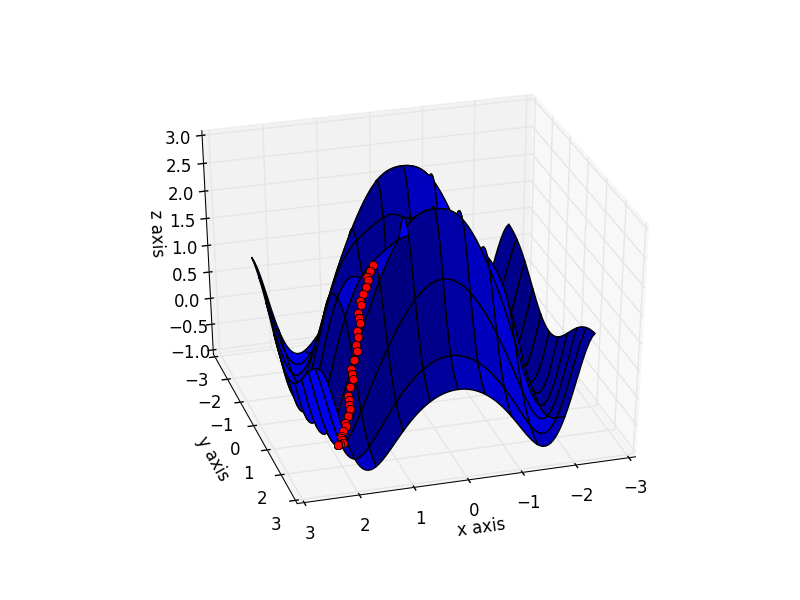
\includegraphics[scale=.5]{figure2.png}
  \caption{Graph with Hill Climbing Path (rotated slightly)}
\end{figure}

Output from this test run:

Hill Climbing Results - x =  1.938238458226389  y =  1.4617642423981192  z =  -0.9394034055128205

\section{Thoughts on Project}
One of the tricky parts of this project was getting the logic correct for the hill climbing algorithm. I had some serious logic errors in my hill climbing’s decision making, which I luckily caught while I was reviewing the code after getting some strange results. Another part that had me sit down and think was the probability portion of the simulated annealing algorithm. A lot of the examples of simulated annealing on the internet were trying to find global maximums, so I had to sit down and think about the formula for the probability of making a move to make sure it was correct for global minimums.



\end{document}
